\chapter{研究过程}
\section{对不同乐器频谱图的分析}
为了研究自然现象和科学模型的关系,我们首先选取了研究声波的手段之一——频谱图来进行分析,我们对五种乐器——大提琴,钢琴,吉他,琵琶,萨克斯风进行了基于傅里叶变换的分析,得到了如下的频率—分贝的频谱图。
\begin{center}
    \vspace{1cm}
    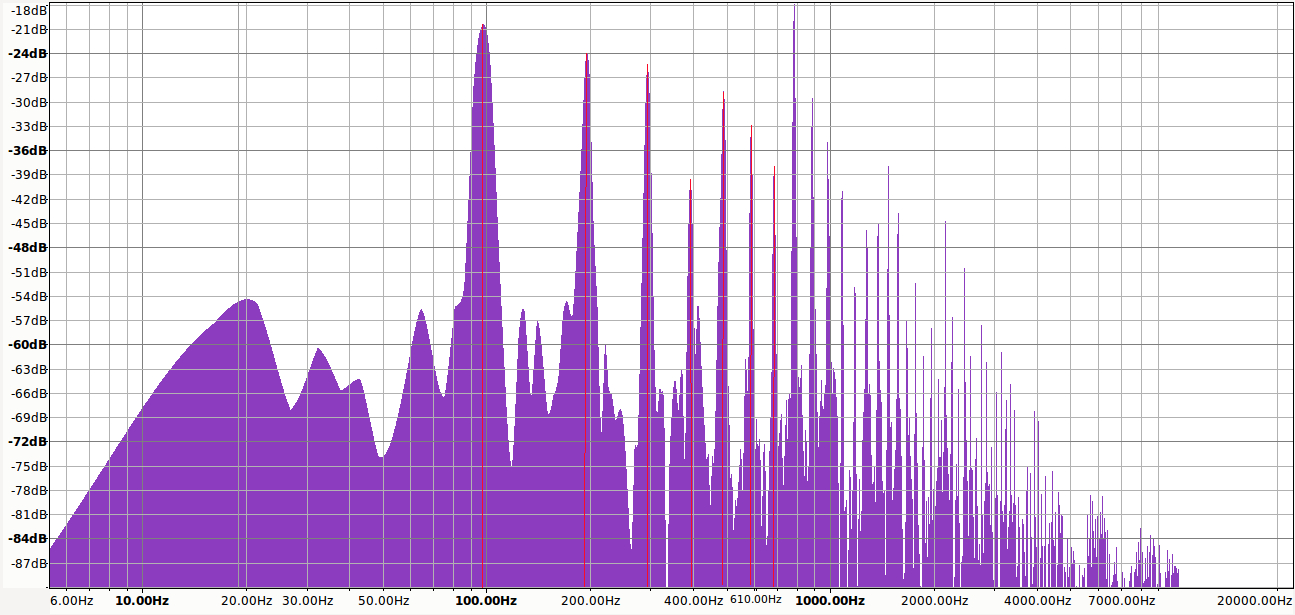
\includegraphics[height=6cm]{cello(G2).jpg}
    \vspace{3mm}
    大提琴(G2)
\end{center}
\begin{center}
    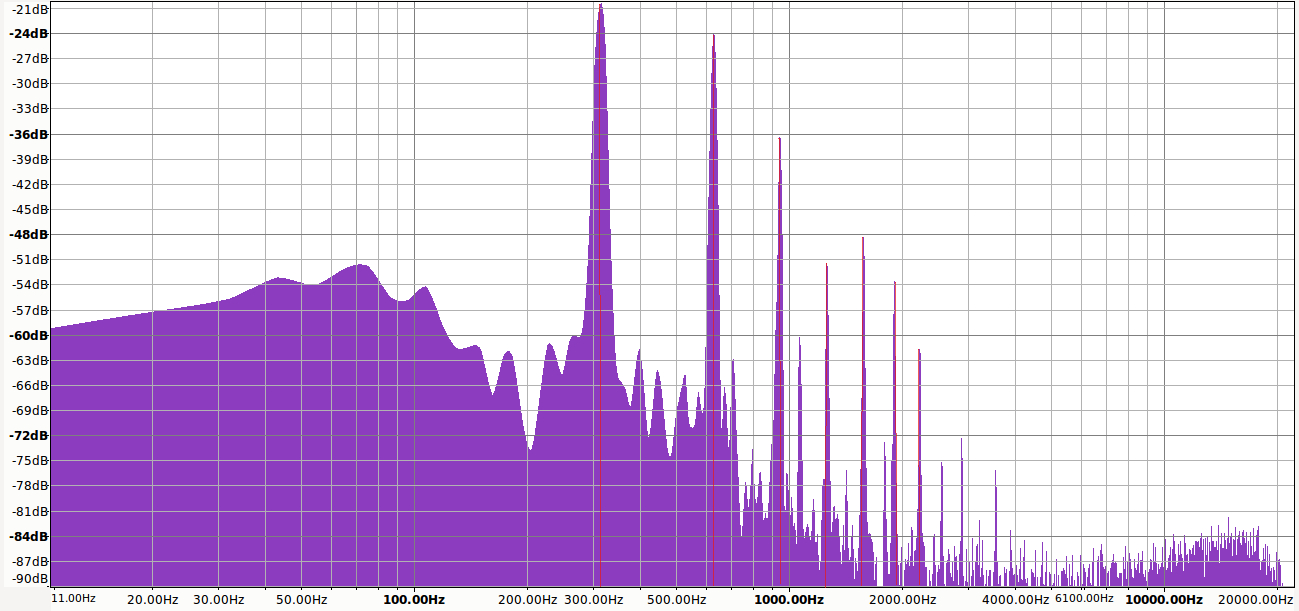
\includegraphics[height=6cm]{piano(D4sharp).jpg}
    \vspace{3mm}
    钢琴(D\#4)
    \vspace{2cm}
\end{center}
\begin{center}
    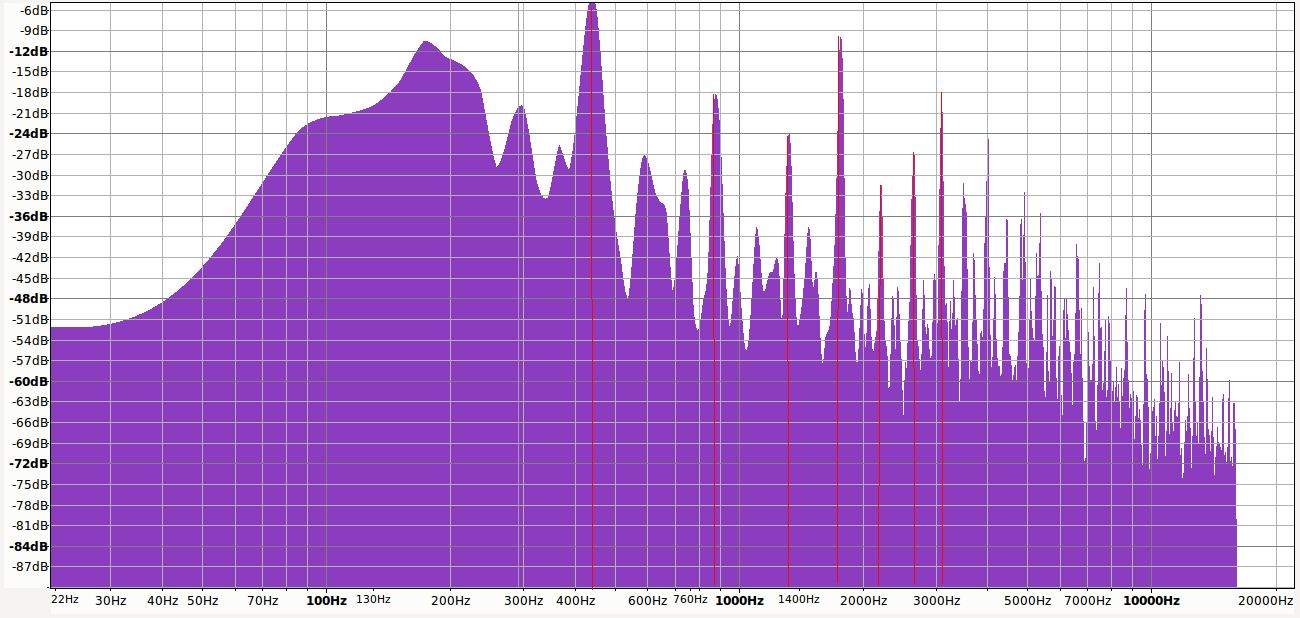
\includegraphics[height=6cm]{guitar(A4).jpg}
    \vspace{3mm}
    吉他(A4)
\end{center}
\begin{center}
    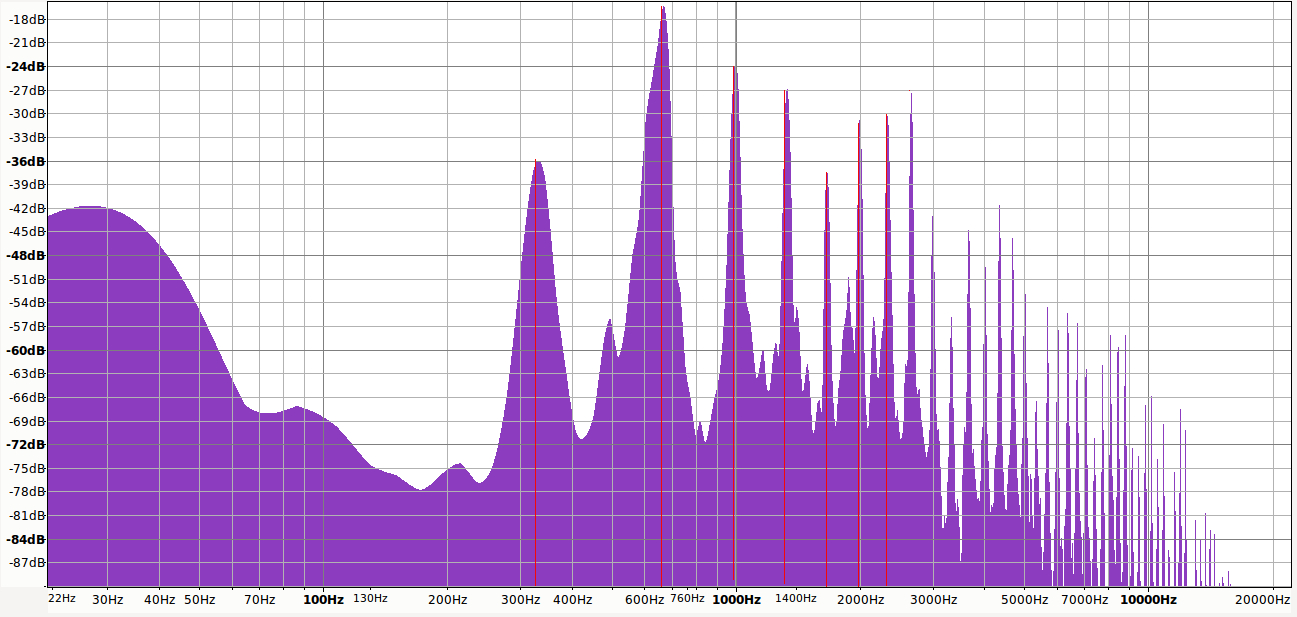
\includegraphics[height=6cm]{lute(E4).jpg}
    \vspace{3mm}
    琵琶(E4)
    \vspace{2cm}
\end{center}
\begin{center}
    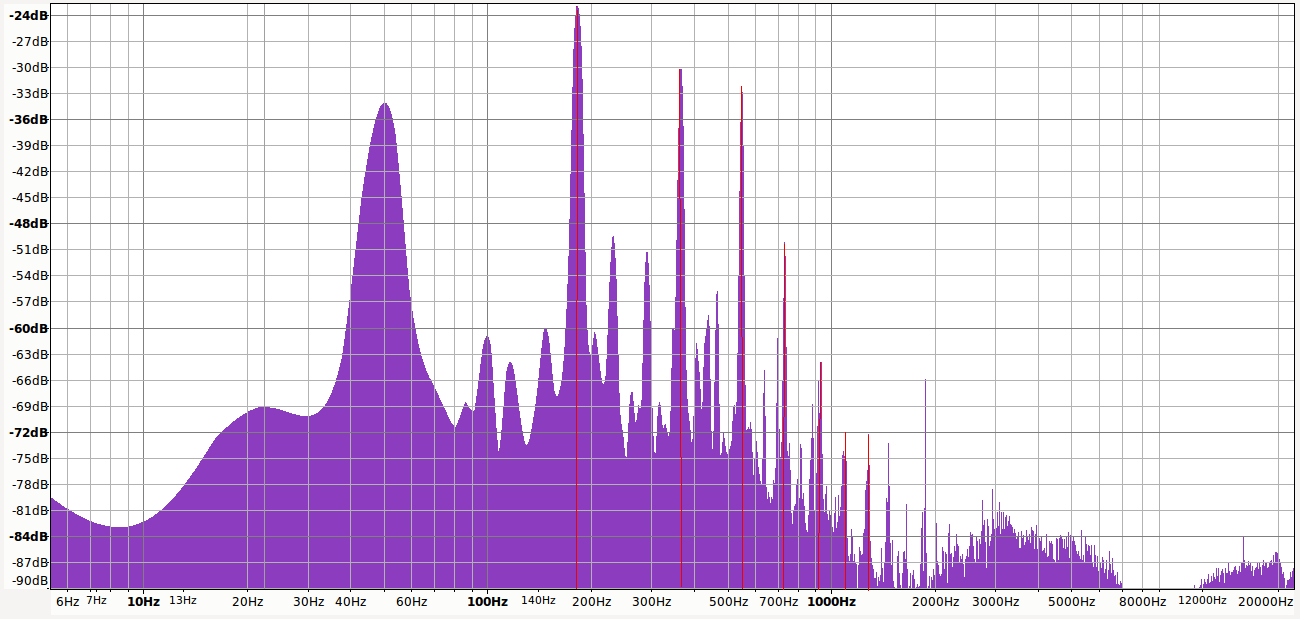
\includegraphics[height=6cm]{saxophone(F3sharp).jpg}
    \vspace{3mm}
    萨克斯风(F\#3)
\end{center}
\par
这些用作实验的乐音是取自网上下载的高保真的音乐专辑,截取单音部分,然后通过波形分析软件Audacity进行分析再绘图得到的。
\par
所选取的五种乐器都是有各阶泛音的弦乐器或管乐器,各阶谐音都用红线标出,为响度的极值点。我们可以看出,各阶泛音的频率确实是基频的整数倍,和书本上所讲述的内容相符。
\par
更进一步的观察可以发现,基频的响度并不一定大于泛音的响度。最典型的例子是琵琶,也就是第四幅图。琵琶素来以泛音丰富饱满,传播很远而闻名。从图中可以看出,琵琶的各阶泛音响度远大于其他乐器。
\section{对用数学模型反映乐音特性的初步思考}
\subsection{对波形的总体观察}
\par
我们知道,要想存储自然界的声音,人们从古至今就想了各种方法。随着科技的发展,当今记录声音的一种手段是波形。但是用波形记录耗费空间巨大。而且出于科学的精神,人们希望有一个简介的模型去体现不同的乐器,于是就有了傅里叶分析这样一些手段,用波的各类特性去记录乐音。
\par
让我们从观察乐器的波形开始,我们选取大提琴作为研究对象。因为大提琴的每个音持续时间较长,平稳饱满,便于观察。
\par
我们首先选取巴赫的无伴奏大提琴组图第一首的起始音(也就是上一节五幅图中的第一幅对应的音)和结束音进行观察。
\vspace{1cm}
\begin{center}
    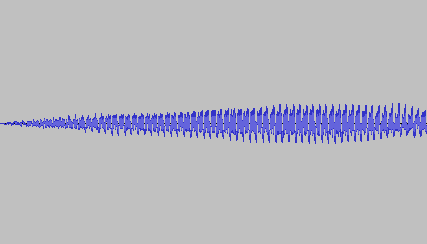
\includegraphics[height=6cm]{celloFirst.png}

    起始音
\end{center}
\vspace{1cm}
\begin{center}
    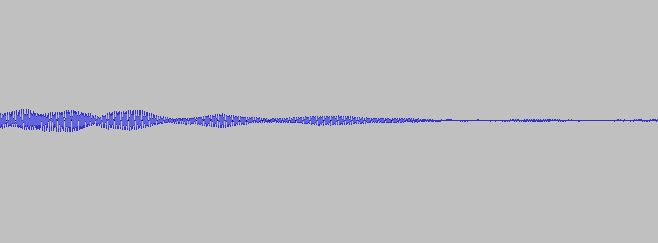
\includegraphics[height=4.2cm]{celloLast.png}

    终止音
\end{center}
\vspace{2cm}
\par
我们可以看出,起始音渐强,终止音减弱,从整体形状上来看很不一样。
\subsection{对波形的细致观察}
\par
我们首先需要审视的是一个稳定的音,我们选取起始音的稳定部分
\vspace{1cm}
\begin{center}
    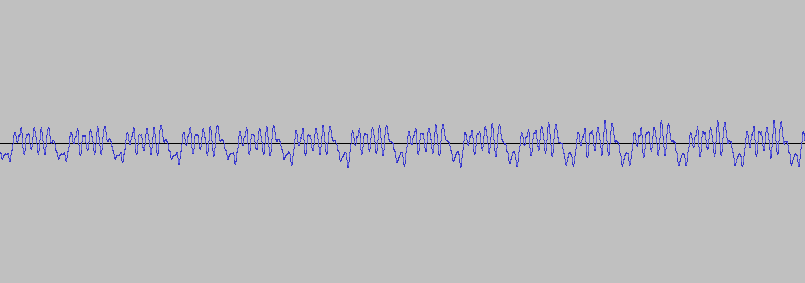
\includegraphics[height=4.2cm]{celloFirstStable.png}
\end{center}
\vspace{1cm}
\par
\vspace{1cm}
我们可以发现,这是一个周期性十分强的图像,它的一个周期内的图像如下
\vspace{1cm}
\begin{center}
    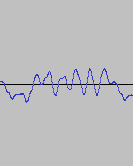
\includegraphics[height=4.2cm]{celloFirstStableBig.png}
\end{center}
\vspace{1cm}
\par
简言之,一个大提琴的音G2的稳定部分就可以用这样一个图像完全的表达,我们现在可以大胆放心的称这幅图为稳定的大提琴的G2。也就是说如果人耳持续不断的接受这样的波形,就会认为听到了巴赫无伴奏组曲第一首的第一个音。
\par
接下来我们来思考一个问题,对于同一件乐器来说,不同音高的音虽然频率不同,但是不是“形状”都一样呢?是不是有可能音调高的音只是音调低的音的波形“压缩”而成呢?如果是这样,岂不是只要一幅图像就可以代表一件乐器的稳定音部分了?
\par
很遗憾,现实并不是如此,我们选取另一个音高比较高的稳定音的局部图与先前的对照
\vspace{1cm}
\begin{center}
    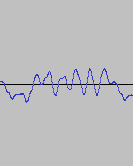
\includegraphics[height=4.2cm]{celloFirstStableBig.png}
    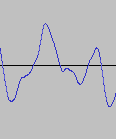
\includegraphics[height=4.2cm]{anotherNoteBig.png}
\end{center}
\vspace{1cm}
\par
我们发现,音高低的音波形比较复杂,音高高的音波形比较单一,两个波形不要说相似了,实在是相差甚远。
\par 
现在我们可以得出一个初步结论,光要记录稳定音,就要记录不同音高的音的波形。但是问题还不止如此。每个音的起始部分和延音部分并不像我们想的那么简单。
\par
我们先来观察第一个音的起始部分
\vspace{1cm}
\begin{center}
    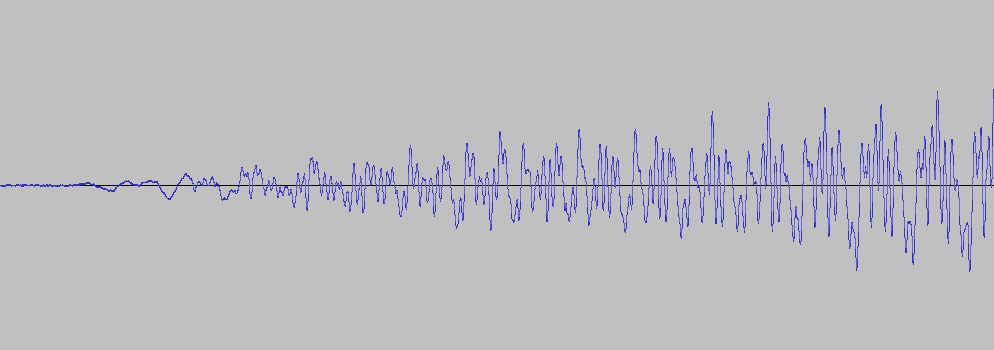
\includegraphics[height=4.2cm]{celloFirstScale.png}
\end{center}
\vspace{1cm}
\par
我们可以看出,一个音的起始,从极端的不规律到稍稍有规律最终才达到平稳音阶段
\par 
再来观察最后一个音的延音部分
\vspace{1cm}
\begin{center}
    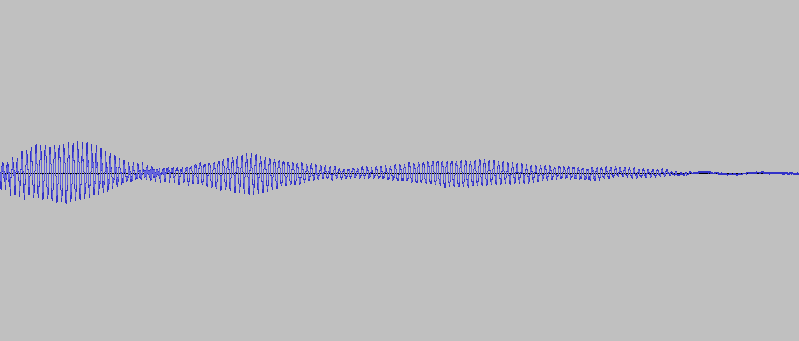
\includegraphics[height=4.2cm]{celloLastScale.png}
\end{center}
\vspace{1cm}
\par
我们发现,和起始音的极端不规律不同,延音部分十分有规律,只是振幅不断震荡并不断变小而已。
\par
对于用波形记录一件乐器,除了要记录每一个音高的音的稳定部分,起始部分,延音部分,还要注意处理两个音交叉的部分,一个音奏响了之后可能会影响之后的几个音,所以还要记录好每个音会延长多长时间,即向后的影响范围是多少。
\section{对人耳区分音高的一些探究}
\par
现在让我们转而来思考另一些问题,给你一段稳定的音频,你是如何区分里面包含了同一个音高的音还是不同音高的音,如果只有同一音高的音,你是如何判断是不是一种乐器发出的,如果只有一种乐器,你是如何判断音高的。
\par 
我们首先来研究第三个问题,我们还是使用之前的素材,研究大提琴G2这个音。我们画出G2的正弦波的图,也就是98Hz的正弦波的图, 与大提琴的波形对照。
\vspace{1cm}
\begin{center}
    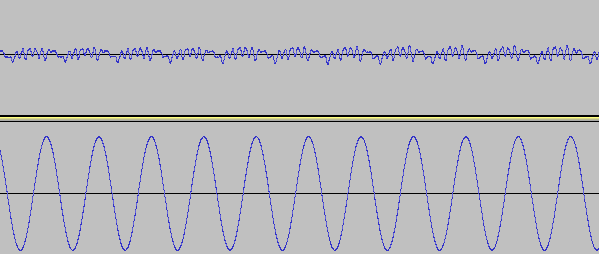
\includegraphics[height=4.2cm]{compare.png}
\end{center}
\vspace{1cm}
\par
我们发现98Hz正弦波的周期正好对应了G2波形的最小正周期。从人耳的角度讲,耳膜持续受到最小正周期形状的波的振动,就会感觉和听98Hz正弦波听到的是同一个音高的音。再进行了几组实验,发现了同样的规律,于是我们可以说,一个单音波形的音高通常由它的最小正周期决定。
\par
接下来我们来思考第二个问题。由于刚刚分析完第一个问题,我们不自然的会想到这样一种情形,如果一个400Hz的音和一个660Hz的音同时奏响,合成的波形的最小正周期应该和一个220Hz的音相同,那么我们真的会听到220Hz的音吗?
\par
通过实验,很不幸,我们并没有听到。但是在网上查阅资料后,发现了一个有趣的现象。
\par
有一种现象称之为消失的基频。最初由巴洛克时期威尼斯的小提琴家兼作曲家塔替尼(G. Tartini)发现,所以后人又称此现象为塔替尼效应(Tartini Effect)。 塔替尼在演奏小提琴时发现,当他用力演奏双音时,会听到一个低音,举个例子,A4(440Hz) + C\#6(1100Hz) ,频率比为2:5,此时会听到A3(220Hz)的声音。\footnote{摘自中文维基百科``消失的基频''词条}
\par
消失的基频(missing fundamental)是心理声学(psychoacoustics)领域常被谈论的现象。周期讯号的基频即为讯号的音高,但基频讯号的强度大小却不一定大过泛音强度大小,有时基频讯号的强度大小甚至为零,这种情形即为我们所谓的消失的基频。 在日常生活中,一般的乐器的声音均是由基频与倍频(泛音)组合而成,而基频就是影响声音音高的主要因素之一。然而,当我们将基频的强度以人为得方式调整为零时,会发现被调整过后的声音音高仍旧不变。 此一现象虽然让音高在频谱上的判别更加困难,但也被应用于讯号处理领域。\footnote{同上}
\par
我们可以来看一个例子,观察下图\footnote{摘自http://auditoryneuroscience.com}
\vspace{1cm}
\begin{center}
    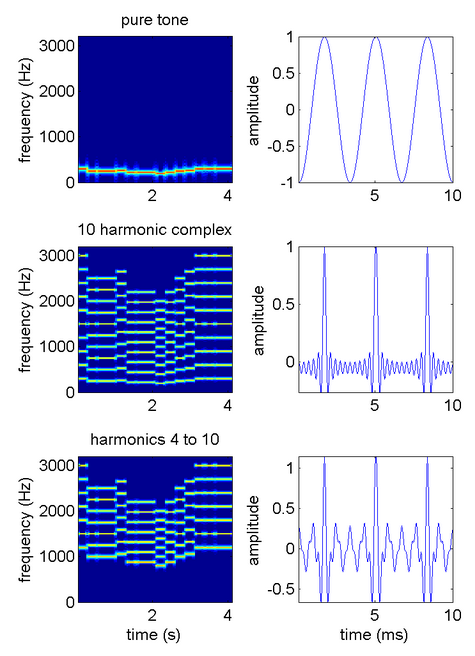
\includegraphics[height=12cm]{triple.png}
\end{center}
\vspace{1cm}
\par 
从图中我们可以看出,即使去掉基音和第二与第三阶谐音,也能“听出”基音来。而这三幅图表达了同一音高的原因是它们的最小正周期相同。看来,要想听到“消失的基音”,还需要比较多的泛音来“突出”它们的最大公约频率。
\par
在百科上关于消失的基音还有几个例子,比如一般的市内电话较难传送频率300Hz以下的讯号,但成年男性的声音大多落在150Hz左右,但成年男性的声音并不会因为经由电话传输过后变得不像男声或是失去磁性。这是由于我们对音高的感知并不会因为基频消失而改变。另外,管风琴为一个占空间的乐器,有时候会因为空间与成本的因素,将乐器最低的那个八度的琴键移除,若是要演奏那些被移除的音,则可以演奏该音的两个泛音,此时聆听者即会听到那个低音,当然这算是幻觉。\footnote{摘自中文维基百科``消失的基频''词条}
\par
让我们再回到同时听两个音的问题来,在大部分情况下,两个频率的最大公约频率很低,响度也很小,人耳很难听出。所以这时人耳无法把听到的频率解释为单一泛音列,所以会去分析其它容易听出的周期。
\par
下面我们做一个实验,将440Hz的正弦波和660Hz的正弦波合成,得到如下的图像。
\vspace{1cm}
\begin{center}
    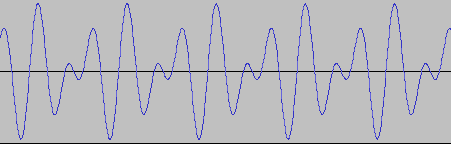
\includegraphics[height=3cm]{mix.png}
\end{center}
\vspace{1cm}
通过播放这段波形,我们发现可以清楚的听到440Hz和660Hz两种不同的声音,我们不禁要问自己,就进是什么是我们的耳朵可以对于这样一种波形辨析出两种不同的频率?
下面试着做一种解释:首先我们可以从混合波形中找到很想440Hz的部分
\begin{center}
    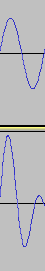
\includegraphics[height=6cm]{440.png}
\end{center}
也可以找到很像660Hz的部分
\begin{center}
    
\includegraphics[height=5cm]{660.png}
\end{center}
所以对人耳来说,感应到了两种不同的周期,就区分出了两种不同的频率。
\par
当然,这个观点只是我们的猜测,可能有道理,也可能不怎么对,当然,本着探究的精神,还是在这里把这种推测提出。
\par
最后我们来看第一个问题,对于不同的乐器同时奏响,人耳如何区分。首先像提琴和钢琴之间音的长短差异巨大,很容易就能从音的持续时间听出差异。而比如说萨克斯风和提琴一起奏同一个音,由于萨克斯声音波动很大,也很容易区分出来。总结就是,不同的乐器除频率组成以外的特质十分明显,人们可以从乐器的其他特质来辨别出来。
\section{对音乐数字化的进一步思考}
\subsection{音乐数字化的方式}
\par
第二节已经分析了要想数字化音乐并没有想象中的那么单纯,乐器奏出的美妙音乐很难用简单的一些函数来还原。
\par
MIDI(Musical Instrument Digital Interface)乐器数字接口 ,是20 世纪80 年代初为解决电声乐器之间的通信问题而提出的。MIDI 传输的不是声音信号, 而是音符、控制参数等指令, 它指示MIDI 设备要做什么,怎么做, 如演奏哪个音符、多大音量等。它们被统一表示成MIDI 消息(MIDI Message) 。传输时采用异步串行通信, 标准通信波特率为31.25×( 1±0.01) KBaud。\footnote{摘自百度百科“MIDI”词条}
\par
最初的合成技术采用FM合成技术,也就是频率调变合成技术,它采用了我们一开始设想的用简单的模型来定义乐音的思想,但是效果差强人意,乐器演奏出的乐音差别甚远,不能令人们满意。后来发展出了波表合成技术。
\par
波表的英文名称为“WAVE TABLE”,从字面翻译就是“波形表格”的意思。其实它是将各种真实乐器所能发出的所有声音(包括各个音域、声调)录制下来,存贮为一个波表文件。播放时,根据MIDI文件纪录的乐曲信息向波表发出指令,从“表格”中逐一找出对应的声音信息,经过合成、加工后回放出来。由于它采用的是真实乐器的采样,所以效果自然要好于FM。一般波表的乐器声音信息都以44.1KHz、16 Bit 的精度录制,以达到最真实回放效果。\footnote{摘自“波表合成技术纵横谈”}
\par 
在制作波表时,要对不同乐器每个音高的音,包括起始部分,稳定部分,和延音部分进行采样,还要采样特殊效果,才能做出一个合格的波表。
\subsection{音乐与听感}
现在我们来讨论最后一个比较哲学的问题,为什么我们会用厚重,清亮,饱满这类词去形容声音呢?根据我们的讨论,我们试着做如下的解释:这些形容声音的词语都是来源于生活的。比如我们听到“厚重低沉”的声音会想到拖拉机轰轰的声响,听到“清亮”的声音会想到敲击玻璃杯的声音,我们认为声音“饱满”是因为我们形容完整的不破损的东西通常用饱满来形容。所以可以说,这些形容声音的形容词都是和生活经历相联系的,并不是声音本身的属性。
